\subsection{Unendliche Reihen} 
\subsubsection{Grundbegriffe}\label{2.1.3}
\paragraph{Def. 6:} 
Gegeben sei die Zahlenfolge $(a_n)_n \geq n_0, \; n\in \mathbb{N}$. Die Zahlenfolge $(S_n)_n \geq n_0$ mit $S_{n_0}:=a_{n_0}, \; S_{n_0 + 1} := a_{n_0}+a_{n_0 +1}, \; S_{n_0 +2} := a_{n_0} + a_{n_0 +1} + a_{n_0 +2}, \; ..., \; S_n=a_{n_0}+a_{n_0 +1} +...+a_n$ (\emph{Partialsumeenfolge}) heißt \emph{unendliche Reihe}.\\
Bezeichnung: $\boxed{\sum_{n=n_0}^{\infty} a_n}$
\begin{itemize}
\item Die Zahlen $a_n$ heißen Glieder der Reihe, die Zahlen $S_n$ heißen Partialsummen der Reihe
\item Ist die Reihe konvergent, d.h. die Folge $(S_n)$ ist konvergent, so heißt $s:=\lim_{n\to \infty}S_n=: \sum_{n=n_0}^{\infty} a_n$ die Summe der Reihe
\item Die Reihe heißt (bestimmt oder unbestimmt) divergent, wenn die Partialsummen die entsprechende Eigenschaft haben.
\end{itemize}
Bemerkung: Oft $n_0=0$ oder $=1$
\subparagraph{Bsp. 6:} $a_n=a q^n$ mit $a\not = 0, q \not = 0, n=0,1,2,...$\\
$(a_n)=(a, aq, aq^2, aq^3,...)$ (\emph{geometrische Zahlenfolge})\\
$(S_n)=\sum_{n=0}^\infty aq^n$ (\emph{geometrische Reihe})\\
$= (\underbrace{a}_{s_0}, \underbrace{a+aq}_{s_1}, \underbrace{a+ aq+ aq^2}_{s_2}, ...)$\\
$S_n=a + aq + aq^2 + aq^3+...+aq^n \quad | \cdot q$\\
$S_nq=aq+aq^2+aq^3+aq^4+...+aq^{n+1}$\\
Beide Zeilen voneinander abgezogen:\\
$S_n-S_nq = a - aq^{n+1}\\
S_n(1-q) = a - aq^{n+1} \quad | : (1-q) \text{ falls }q\not = 1\\
\boxed{S_n = a\cdot \frac{1-q^{n+1}}{1-q}}$ (\emph{Summenformel für die endliche geometrische Reihe} mit Anfangsglied $a$ und $n+1$ Summanden)\\
$\Rightarrow \lim_{n\to \infty}S_n=\frac{a}{a-q}$ falls $|q|<1$
$\Rightarrow$ Summe der unendlichen geometrischen Reihe:\\
$\boxed{\sum_{n=0}^\infty a q^n=\frac{a}{1-q}}$ für $|q|<1$.\\
z.B. $0,\overline{72}=0,727272...=\frac{72}{100}+\frac{72}{10.000}+\frac{72}{1.000.000}+...=\frac{72}{99}=\frac{8}{11}$

\subparagraph{Bsp. 7:} $\sum_{n=1}^\infty \frac{1}{n}=1+\frac{1}{2}+\frac{1}{3}+...$ heißt \emph{harmonische Reihe}. Offensichtlich ist $(S_n)$ streng monoton wachsend. Man kann zeigen, dass $(S_n)$ nicht beschränkt ist. Aus Satz 3 folgt: die harmonische Reihe ist bestimmt divergent.\\
Schreibweise: $\sum_{n=1}^\infty \frac{1}{n}=\infty$

\paragraph{Def. 7:} Die Reihe $\sum_{n=n_0}^\infty a_n$ heißt
\begin{enumerate}[label=(\alph*)]
\item absolut konvergent, falls $\sum_{n=n_0}^\infty|a_n|$ konvergent ist.
\item bedingt konvergent, falls $\sum_{n=n_0}^\infty a_n$ konvergent, aber $\sum_{n=n_0}^\infty |a|$ nicht konvergent ist.
\end{enumerate}

\paragraph{Satz 5:} $\sum_{n=n_0}^\infty a_n$ absolut konvergent $\Rightarrow$ $\sum_{n=n_0}^\infty a_n$ konvergent.
\subparagraph{Diskussion:}
\begin{enumerate}
\item Die Umkehrung gilt im Allgemeinen nicht. Es gibt konvergente Reihen, die nicht absolut konvergieren. Z.B. $\sum_{n=1}^\infty (-1)^{n-1}\frac{1}{n}=1-\frac{1}{2}+\frac{1}{3}-\frac{1}{4}+...$
\item Für Reihen mit nicht-negativen Gliedern ($a_n \geq 0$ für alle $n$) ist absolute Konvergenz identisch mit (gewöhnlicher) Konvergenz. Für solche Reihen gilt entweder $\sum_{n=n_0}^\infty a_n<\infty$ [(absolut) konvergent] oder $\sum_{n=n_0}^\infty a_n = \infty$ [bestimmt divergent].
\end{enumerate}

\subsubsection{Konvergenzkriterien}
\begin{enumerate} [label= \arabic*., wide]
\item Notwendiges Konvergenzkriterium
\paragraph{Satz 6:} $\sum_{n=n_0}^\infty a_n$ konv. $\Rightarrow$ $\lim_{n\to \infty} a_n = 0$\\
bzw.: $(a_n)$ konvergiert $\Rightarrow$ $\sum_{n=0}^\infty a_n$ divergiert 
\subparagraph{Beweis:} $a_n = S_n - S_{n-1}$\\
$\Rightarrow \lim_{n\to \infty}a_n = \lim_{n\to\infty}S_n - \lim_{n\to\infty}S_{n-1}=s-s=0$
\subparagraph{Bemerkung:} 
\begin{enumerate}
\item Bedingung $\lim_{n\to\infty}a_n = 0$ ist notwendig, aber nicht hinreichend. Z.B. $a_n=\frac{1}{n}$, dann $\lim_{n\to\infty}a_n=0$ aber $\sum_{n=1}^\infty a_n=\infty$
\item Anwendung des Satzes meist in logisch äquivalenter Form: $\lim_{n \to \infty} a_n \not = 0 \Rightarrow \sum_{n=n_0}^\infty a_n$ divergiert
\end{enumerate}

\subparagraph{Bsp. 8:} $\sum_{n=1}^\infty \left(\frac{n}{10n-1}\right)^{50}$\\
$a_1=1,94\cdot 10^{-48}, a_2=1,3 \cdot 10^{-49}, ...$\\
$\lim_{n\to\infty}a_n=\lim_{n\to\infty}\left(\frac{n}{10-\frac{1}{n}}\right)^{50}\not = 0$\\
$\Rightarrow$ Reihe divergent (sogar besimmt divergent, da alle $a_n \geq 0$)

\item Hinreichendes Kriterien
\begin{enumerate}[label=(\Alph*),wide]
\item \emph{Leibnitzkriterium für alternierende Reihen}
\paragraph{Satz 7:} Sei $(b_n)$ Folge mit 
\begin{itemize}
\item $b_n \geq b_{n+1} > 0$ für alle $n \in \mathbb{N}$
\item $\lim_{n\to\infty} b_n = 0$
\end{itemize}
Dann ist $\sum_{n=0}^\infty(-1)^n b_n=b_0-b_1+b_2-b_3+...$ konvergent. D.h. wenn die Beträge $b_n$ der Glieder einer alternierenden Reihe mit $a_n = (-1)^n b_n$ eine Nullfolge bilden, dann ist die Reihe konvergent.\\
Weiter gilt: $|s-S_n| \leq | a_{n+1} |$\\
Also ist der Fehler bei der Approximation von $s$ durch $S_n$ beschränkt durch den Beträg von $a_{n+1}$.

\subparagraph{Bsp. 9:} $\sum_{n=1}^\infty (-1)^{n-1} \frac{1}{n}=1-\frac{1}{2}+\frac{1}{3}-\frac{1}{4}+...$ (alternierende harmonische Reihe)\\
$s_1=1, \; s_2=0,5, \; s_3\approx 0,83, \; s_4\approx 0,583, \; s_5\approx 0,78, \; s_6\approx 0,62$\\
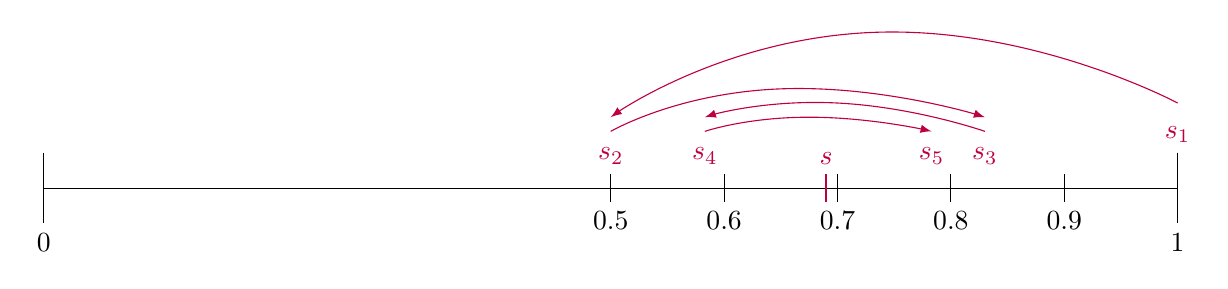
\begin{tikzpicture}[scale=.9]
\draw (0,0) -- (16,0);
\foreach \x in {0,1}{
	\draw (\x*16, 0.5) -- (\x*16,-0.5) node[below]{$\x$};
}
\foreach \x in {0.5,0.6,0.7,0.8,0.9}{
	\draw (\x*16, 0.2) -- (\x*16,-0.2) node[below]{$\x$};
}

\node[above, purple] at (16,0.5) {$s_1$};
\node[above, purple] at (0.5*16,0.2) {$s_2$};
\node[above, purple] at (0.83*16,0.2) {$s_3$};
\node[above, purple] at (0.583*16,0.2) {$s_4$};
\node[above, purple] at (0.783*16,0.2) {$s_5$};

\node[above, purple] at (0.69*16,0.2) {$s$};
\draw[purple, thick] (0.69*16, 0.2) -- (0.69*16,-0.2);

\draw [-latex, purple] plot[smooth, tension=1] coordinates {(16,1.2) (11.8,2.2) (8,1)};
\draw [-latex, purple] plot[smooth, tension=1] coordinates {(8,0.8) (10.4,1.4) (0.83*16,1)};
\draw [-latex, purple] plot[smooth, tension=1] coordinates {(0.83*16,0.8) (11.2,1.2) (0.583*16,1)};
\draw [-latex, purple] plot[smooth, tension=1] coordinates {(0.583*16,0.8) (10.8,1) (0.783*16,0.8)};
\end{tikzpicture}\\
Man kann zeigen: $s=\ln 2 = 0,6931$
\item \emph{Verleichskriterien für Reihen mit nicht-negativen Gliedern}
\paragraph{Satz 8:} (Majoranten-Kriterium)\\
Seien $(a_n)_{n\geq n_0}, (b_n)_{n\geq n_0}$ Folgen mit $0 \leq a_n \leq b_n$ für alle $n\geq n_1 \geq n_0$ und $\sum_{n=n_0}^\infty b_n < \infty$ (d.h. konvergent). \\
Dann $\sum_{n=n_0}^\infty a_n < \infty$ (d.h. konvergent).

Die Reihe $\sum _{n=n_0}^\infty b_n$ heißt dann konvergente Majorante zur Reihe $\sum_{n=n_0}^\infty a_n$.\\
Beweisidee: $0\leq a_n \leq b_n \rightsquigarrow 0 \leq \sum _{n=n_0}^\infty a_n \leq \sum _{n=n_0}^\infty b_n \leq \infty $
\paragraph{Satz 9:} (Minoranten-Kriterium)\\
Seien $(a_n)_{n\geq n_0}, (b_n)_{n\geq n_0}$ Folgen mit $0 \leq b_n \leq a_n$ für $n\geq n_1 \geq n_0$ und $\sum_{n=n_0}^\infty b_n = \infty$ (d.h. divergent)\\
Dann $\sum_{n=n_0}^\infty a_n = \infty$ (also auch divergent)\\
Die Reihe $\sum_{n=n_0}^\infty b_n$ heißt divergente Minorante der Reihe $\sum_{n=n_0}^\infty a_n$.\bigskip\\
Eine nützliche Vergleichsreihe für die Anwendung der Sätze 8 und 9 ist:\\
$\boxed{\sum_{n=1}^\infty \frac{1}{n^\lambda}= \begin{cases}
\text{konvergent} & \text{für }\lambda > 1\\
\text{divergent} & \text{für }\lambda \leq 1
\end{cases}}$
\subparagraph{Bsp. 10:} Man untersuche das Konvergenzverhalten der folgenden Reihe:
\begin{enumerate}[label=\alph*.)]
\item $\sum_{n=1}^\infty \underbrace{\frac{1}{n^2-n+1}}_{a_n}$ (Vermutung: Verhalten wie $\sum \frac{1}{n^2}$ wegen der Dominanz der höchsten Potenz)\\
Wir versuchen eine konvergente Majorante zu finden.\\
$a_n=\frac{1}{n^2-n+1}\geq \frac{1}{n^2-\frac{n^2}{2}}$ (wegen $n\geq \frac{n^2}{2}$ für $n\geq 2$)\\
Somit $\frac{1}{n^2-\frac{n^2}{2}}= \frac{2}{n^2}=:b_n$\\
Mit der Vergleichsreihe gilt: $\sum_{n=1}^\infty b_n = 2 \sum_{n=1}^\infty \frac{1}{n^2}$ ist konvergent.\\
$\overset{\text{Satz 8}}{\Longrightarrow} \sum_{n=0}^\infty a_n$ ist konvergent, sogar absolut konvergent, da $a_n\geq 0 \; (n \in \mathbb{N})$
\item $\sum_{n=1}^\infty \frac{n^2+4}{n^3+n^2+31}$ (Vermutung: divergent, da Verhalten wie $\sum \frac{n^2}{n^3}=\sum \frac{1}{n}$)\\
Wir versuchen divergente Minoranten zu finden.\\
$a_n = \frac{n^2+4}{n^3+n^2+31}\geq ... \geq \frac{1}{3n}=: b_n$ (für $n\geq 4$)\\
Wieder gilt mit der Vergleichsreihe: $\sum b_n$ divergent. Also folgt mit Satz 9: $\sum_{n=1}^\infty a_n$ divergent.
\end{enumerate}
\item \emph{Quotienten- und Wurzelkritierien}
\paragraph{Satz 10:} (Quotientenkriterium)\\
Sei $(a_n)_{n\geq n_0}$ eine Folge, so gilt:\\
$\boxed{\lim_{n\to\infty}\left|\frac{a_{n+1}}{a_n}\right|\begin{cases}
<1\\
>1
\end{cases}\Rightarrow \sum_{n=n_0}^\infty a_n \text{ ist}\begin{cases}
\text{absolut konvergent}\\
\text{divergent}
\end{cases}}$
\paragraph{Satz 11:} (Wurzelkriterium)\\
Sei $(a_n)_{n\geq n_0}$ eine Folge, so gilt:\\
$\boxed{\lim_{n\to\infty} \sqrt[n]{|a_n|} \begin{cases}
<1\\
>1
\end{cases}\Rightarrow \sum_{n=n_0}^\infty a_n \text{ ist}\begin{cases}
\text{absolut konvergent}\\
\text{divergent}
\end{cases}}$
\subparagraph{Bemerkung:} Falls in Satz 10 oder 11 $\lim ... =1$ gilt, so ist mit diesem Kriterium keine Konvergenzaussage möglich.

\subparagraph{Bsp. 11:}
\begin{enumerate}[label=\alph*.)]
\item $\sum_{n=2}^\infty \underbrace{\left( \frac{1}{\ln(n)}\right)^n \cdot (-1)^n}_{a_n}$\\
Wegen $\sqrt[n]{|a_n|}=\frac{1}{\ln n} \overset{n\to\infty}{\longrightarrow} 0 $ liefert das Wurzelkriterium, dass die Reihe absolut konvergent ist.
\item $\sum_{n=1}^\infty \frac{(-1)^n (2n)!}{(n!)^2}$\\
Wegen $\left|\frac{a_{n+1}}{a_n}\right|=\frac{\frac{(2(n+1))!}{((n+1)!)^2}}{\frac{(2n)!}{(n!)^2}}=\frac{(2n+2)!}{((n+1)!)^2}\cdot \frac{(n!)^2}{(2n)!}=\frac{(2n+2)(2n+1)(n!)^2}{(n+1)^2 (n!)^2}=\frac{(2n+2)(2n+1)}{(n+1)^2}
=\frac{4n^2+4n+2n+2}{n^2+2n+1}\overset{n\to\infty}{\longrightarrow} 4$\\
Daher ist die Reihe divergent.
\end{enumerate}
\end{enumerate}
\end{enumerate}

\subsubsection{Rechenregeln}
\begin{itemize}
\item $\sum_{n=n_0}^\infty a_n$ und $\sum_{n=n_0}^\infty b_n$ konvergent mit Summe $a$ und $b$, dann gilt: 
\begin{itemize}
\item $\sum_{n=n_0}^\infty (a_n+b_n)= a + b$
\item $\sum_{n=n_0}^\infty c\cdot a_n= c\cdot a$
\end{itemize}
\item $\sum_{n=n_0}^\infty a_n$ absolut konvergent $\Leftrightarrow$ die Glieder $a_n$ lassen sich beliebig umordnen, ohne dass sich die Summe ändert.
\item $\sum_{n=n_0}^\infty a_n$ und $\sum_{n=n_0}^\infty b_n$ absolut konvergent mit Summen $a$ und $b$, dann gilt:
\begin{itemize}
\item $\left(\sum_{i=0}^\infty a_i\right)\cdot \left( \sum_{j=0}^\infty b_j\right)=\sum_{i=0}^\infty  \sum_{j=0}^\infty a_i b_j=a\cdot b \qquad \left( =\sum_{n=0}^\infty  \sum_{i=0}^\infty a_i b_{n-i} \quad \text{Cauchy-Produkt}\right)$
\end{itemize}
\end{itemize}

\section{Grenzwerte und Stetigkeit von Funktionen}
\subsection{Grenzwerte von Funktionen}
\paragraph{Def. 1:} Es sei $x_0 \in \mathbb{R}$ und es existiere eine Umgebung $U(x_0)$ mit $U(x_0)\{x_0\}\subseteq Db(f)$.\\
\begin{tikzpicture}[scale=1]
\draw[-latex] (0.5,0) -- (8.5,0);
\path[pattern= north east lines, pattern color=green] (1.2,0.2) rectangle (3.2,-0.2);
\path[pattern= north east lines, pattern color=green] (4,0.2) rectangle (5.4,-0.2);
\path[pattern= north east lines, pattern color=green] (6.4,0.2) rectangle (7.8,-0.2);
\draw (4.6,0.4) -- (4.6,-0.4) node[below]{$x_0$};
\draw [orange, thick] (4.2,0.01) -- (5,0.01);
\draw [orange, thick] plot[smooth, tension=1] coordinates {(4.3,0.25) (4.2,0) (4.3,-0.25)};
\draw [orange, thick] plot[smooth, tension=1] coordinates {(4.9,0.25) (5,0) (4.9,-0.25)};
\node [above right, orange] at (4.6,0.3) {$U(x_0)$};
\node [right] at (8,0.5) {korrekt};
\end{tikzpicture}\\
\begin{tikzpicture}[scale=1]
\draw[-latex] (0.5,0) -- (8.5,0);
\path[pattern= north east lines, pattern color=green] (2.2,0.2) rectangle (4.52,-0.2);
\path[pattern= north east lines, pattern color=green] (4.68,0.2) rectangle (6.6,-0.2);
\draw (4.6,0.4) -- (4.6,-0.4) node[below]{$x_0$};
\draw [orange, thick] (4.2,0.01) -- (5,0.01);
\draw [orange, thick] plot[smooth, tension=1] coordinates {(4.3,0.25) (4.2,0) (4.3,-0.25)};
\draw [orange, thick] plot[smooth, tension=1] coordinates {(4.9,0.25) (5,0) (4.9,-0.25)};
\node [above right, orange] at (4.6,0.3) {$U(x_0)$};
\node [right] at (8,0.5) {korrekt};
\draw  (4.6,0) ellipse (0.2 and 0.2);
\end{tikzpicture}\\
\begin{tikzpicture}[scale=1]
\draw[-latex] (0.5,0) -- (8.5,0);
\path[pattern= north east lines, pattern color=green] (1.6,0.2) rectangle (3.8,-0.2);
\path[pattern= north east lines, pattern color=green] (6.4,0.2) rectangle (8,-0.2);
\draw (4.6,0.4) -- (4.6,-0.4) node[below]{$x_0$};
\draw [orange, thick] (4.2,0.01) -- (5,0.01);
\draw [orange, thick] plot[smooth, tension=1] coordinates {(4.3,0.25) (4.2,0) (4.3,-0.25)};
\draw [orange, thick] plot[smooth, tension=1] coordinates {(4.9,0.25) (5,0) (4.9,-0.25)};
\node [above right, orange] at (4.6,0.3) {$U(x_0)$};
\node [right] at (8,0.5) {falsch};
\end{tikzpicture}\\
$\lim_{x\to x_0} f(x)=\lambda : \Leftrightarrow$ Für jede Folge $(x_n)$ mit $x_n\in Db(f)$, $x_n \not = x$ (für alle $n$) und $\lim_{n\to\infty}x_n=x_0$ gilt $\lim_{n\to\infty}f(x_n)=a$.\\
Anschaulich: $f(x)$ strebt gegen $a$, wenn $x$ gegen $x_0$ strebt.
\subparagraph{Bemerkung:} Die Stelle $x_0$ muss \emph{nicht} selbst zum Definitionsbereich gehören.
\subparagraph{Bsp. 1:}
\begin{itemize}
\item $\lim_{x\to 0} \frac{\sin(x)}{x}$\\
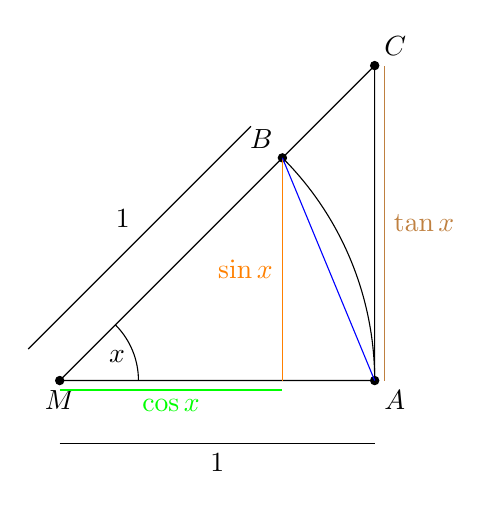
\begin{tikzpicture}[scale=4]

\draw (0,0) -- (1,0) -- (1,1) -- cycle;
\fill  (0,0) circle (0.015) node [below]{$M$};
\fill  (1,0) circle (0.015) node [below right]{$A$};
\fill  (1,1) circle (0.015) node [above right]{$C$};
\fill  (0.707,0.707) circle (0.015) node [above left]{$B$};

\draw [ {[-]} ] (0,-0.2) -- (1,-0.2) node[pos=.5, below]{$1$};
\draw [ {[-]} ] (-0.1,0.1) -- (0.607,0.807) node[pos=.5, above left]{$1$};
\draw (1,0) arc (0:45:1);

\draw (0.25,0) arc (0:45:0.25) node [left, pos=.4]{$x$};
\draw [green] (0,-.03) -- (0.707, -0.03) node[below, pos=.5]{$\cos x$};
\draw [orange] (0.707,0) -- (0.707, 0.707) node[left, pos=.5]{$\sin x$};
\draw [brown] (1.03,0) -- (1.03, 1) node[right, pos=.5]{$\tan x$};
\draw [blue] (0.707,0.707)-- (1,0);
\end{tikzpicture}\\
$F_{\vartriangle MAB}\leq F_{Sektor\; MAB} \leq F_{\vartriangle MAC}$\\
$\frac{1}{2}\sin x < \frac{1}{2} x < \frac{1}{2} \tan x \quad |\cdot \frac{2}{\sin x}$\\
$\Leftrightarrow 1 < \frac{x}{\sin x} < \frac{1}{\cos x}$\\
$\Leftrightarrow 1 > \frac{\sin x}{x} > \cos x$\\
$\Rightarrow \lim_{x\to 0} \frac{\sin(x)}{x}=1$
\end{itemize}
Analog zu Grenzwertsätzen für Zahlenfolgen gilt:
\paragraph{Satz 1:} Es gelte $\lim_{x\to x_0} f(x) = a$ und $\lim_{x\to x_0} g(x) = b$. Dann:
\begin{itemize}
\item $\lim_{x\to x_0} (f(x)+g(x) = a+b$
\item $\lim_{x\to x_0} c \cdot f(x) = c \cdot a$
\item $\lim_{x\to x_0} (f(x) \cdot g(x)) = a \cdot b$
\item $\lim_{x\to x_0}\frac{f(x)}{g(x)}=\frac{a}{b} \quad $ (falls $b\not = 0$)
\end{itemize}
\subparagraph{Bsp. 2:}
\begin{enumerate}[label=\alph*.)]
\item $\lim_{x\to 0} \frac{3x^3-7x+4}{3 \cos x} = \frac{4}{3}$
\item $\lim_{x\to 3} \frac{x^2-x-6}{x-3}=\mq{\frac{0}{0}}$ Satz nicht anwendbar.\\
$= \lim_{x\to 3} \frac{(x-3)(x+2)}{(x-3)} = \lim_{x\to 3} x+2 = 5$\\
(andere Möglichkeit mit $\mq{\frac{0}{0}}$ umzugehen lernen wir später)
\end{enumerate}
\paragraph{Def. 2:} 
\begin{enumerate}[label = \alph*.)]
\item rechtseitiger Grenzwert:\\
$\lim_{x\searrow x_0} f(x)=a : \Leftrightarrow $ für jede Folge $(x_n)$ mit $x_n \in Db(f)$ und $x_n > x_0$ und $\lim_{n\to \infty} x_n =x_0$ gilt $\lim_{n\to \infty} f(x_n)=a$.\\
Andere Schreibweise: $\lim_{x\searrow x_0}=\lim_{x\to x_0+0}$
\begin{tikzpicture}[scale=2]
\draw [-latex] (-0.8, 0) -- (1.7, 0);
\draw (0, 0.1) -- (0,-0.1) node[below]{$x_0$};
\draw (1, 0.1) -- (1,-0.1)node[below]{$x$};
\draw [-latex] (0.9,0.15) -- (0.4,0.15);
\end{tikzpicture}
\item linkseitiger Grenzwert:\\
$\lim_{x\nearrow x_0} f(x) =a :\Leftrightarrow$ analog rechtsseitiger Grenzwert
\item $\lim_{x\to \infty} f(x) = a :\Leftrightarrow$ für jede Folge $(x_n)$ mit $x_n \in Db(f)$ und $\lim_{x\to \infty} x_n = \infty$ gilt $\lim_{n\to \infty} f(x_n)=a$.
\item $\lim_{x\to \infty} f(x) =a :\Leftrightarrow$ analog s.o.
\end{enumerate}
\subparagraph{Diskussion:} Uneigentliche Grenzwerte:\\
Wir schreiben 
 $\lim_{\bullet} f(x) 0 \begin{cases}
 \infty\\
 -\infty
 \end{cases}$  bei bestimmter Divergenz der Funktionswerte für:\\
$\bullet \begin{cases}
x \to x_0\\
x \nearrow x_0\\
x \searrow x_0\\
x\to \infty\\
x\to -\infty
\end{cases}$

\paragraph{Satz 2:}\parskp
$\lim_{x\to x_0} f(x) =a \Leftrightarrow \lim_{x\nearrow x_0} f(x)=\lim_{x\searrow x_0}=a$

\subparagraph{Bsp. 3:} (einseitiger Grenzwert)\\
$f(x)=\begin{cases}
-x^2 & \text{ für } x<0\\
\sqrt{x+1} & \text{ für } x\geq 0
\end{cases}$\\
\begin{tikzpicture}
\draw [thick, domain=0:3] plot[smooth] (\x,{sqrt(\x+1)});
\draw [thick, domain=-1.5:0] plot[smooth] (\x,{-(\x*\x)});
\draw (0,0) circle(0.1);
\fill (0,1) circle(0.1);

\draw [-latex] (-3.2,0) -- (3.2,0) node [below right] {$x$};
\draw [-latex] (0,-2.2) -- (0,2.2) node [above right] {$y$};
\end{tikzpicture}\\
$\lim_{x\nearrow 0}f(x) = 0, \; \lim_{x\searrow 0}f(x)=1$\\
$\Rightarrow \lim_{x\to 0}f(x)$ existiert nicht!

\paragraph{Bsp. 4:} \parskp
$\lim_{x\to \infty} x \cdot \sin \left(\frac{4}{x}\right)= \mq{\infty \cdot 0}$\\
$\overset{u=\frac{4}{x}}{=}\lim_{u\searrow 0}\frac{4}{u} \sin(u) = 4$
\paragraph{Bsp. 5:} \parskp
$\lim_{x\nearrow \frac{\pi}{2}} \tan x = \infty$\\
$\lim_{x\searrow \frac{\pi}{2}} \tan x = -\infty$\\
\begin{tikzpicture}[scale = 0.5]
\draw plot [domain=(3.15-1.3):(3.15+1.3)] (\x, {tan(\x r)} );
\draw plot [domain=(-1.3):(1.3)] (\x, {tan(\x r)} );
%\draw [dashed] ((0.5*3.14),-3) -- ((0.5*3.14),3); 
\draw [dashed] (1.56, -4) -- (1.56, 4);
\draw [thick] (1.56, 0.5) -- (1.56, -0.5) node [below left]{$\frac{\pi}{2}$};

\draw [-latex] (-3.2*2,0) -- (3.2*2,0) node [below right] {$x$};
\draw [-latex] (0,-2.2*2) -- (0,2.2*2) node [above right] {$y$};
\end{tikzpicture}
\subsection{Stetigkeit von Funktionen}
\paragraph{Def. 3:} Sei $f: Db(f)\to \mathbb{R}, \; Db(f) \subseteq \mathbb{R}$ eine Funktion und $x_0 \in Db(f)$ gegeben.\\
Es heißt $f$:
\begin{enumerate}[label=\alph*.)]
\item stetig in $x_0$ falls $\lim_{x \to x_0} f(x) = f(x_0)$ gilt\\
(also $\lim_{x\to x_0} f(x)=f(\lim_{x\to x_0}x)$, d.h. Limes und Funktion kann vertauscht werden).\\
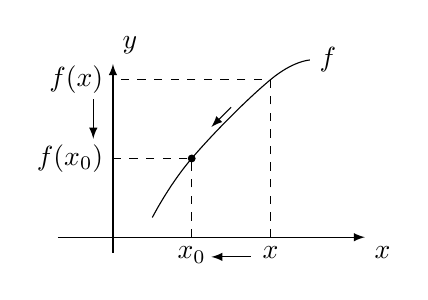
\begin{tikzpicture}[scale = 0.5];
\draw  plot[smooth, tension=.7] coordinates {(1,.5) (2,2) (4,4) (5,4.5)} node[right] {$f$};
\fill (2,2) circle (.1);
\draw [latex-]( 2.5, 2.8)--(3,3.3);
\draw[dashed] (2,0) node[below]{$x_0$}-- (2,2) -- (0,2) node[left]{$f(x_0)$};
\draw[dashed] (4,0) node[below]{$x$} -- (4,4) -- (0,4) node[left]{$f(x)$};

\draw [-latex] (-1.4,0) -- (6.4,0) node [below right] {$x$};
\draw [-latex] (0,-0.4) -- (0,4.4) node [above right] {$y$};
\draw [-latex] (3.5,-0.5) -- (2.5,-0.5);
\draw [-latex] (-0.5,3.5) -- (-0.5,2.5);
\end{tikzpicture}
\item linksseitig stetig in $x_0$, falls $\lim_{x\nearrow x_0}f(x)=f(x_0)$.
\item rechtsseitig stetig in $x_0$, falls $\lim_{x\searrow x_0}f(x)=f(x_0)$.
\end{enumerate}

\subparagraph{Bsp. 6:}
\begin{enumerate}[label=\alph*.)]
\item $f_1(x)=\begin{cases}
\frac{\sin x}{x} & x\not = 0 \\
0 & x = 0
\end{cases}$ ist in $x_0=0$ nicht stetig, da $\lim_{x\to 0} f(x) = 1 \not = 0 = f(0)$.\\
Aber $\overset{\sim}{f}_1(x)=\begin{cases}
f(x) & x\not = 0\\
1 & x= 0
\end{cases}$ ist in $x_0=0$ stetig.\\
Bezeichnung: hebbare Unstetigkeit.\\
\begin{tikzpicture}[scale = 0.5]
\draw [-latex] (-6.4,0) -- (6.4,0) node [below right] {$x$};
\draw [-latex] (0,-4.4) -- (0,4.4) node [above right] {$y$};
\draw plot[domain=-5:-0.2, smooth] (\x, {4.12*sin(50*\x)/\x});
\draw plot[domain=0.2:5, smooth] (\x, {4.12*sin(50*\x)/\x});
\draw  (0,3.6) circle (0.2) node[above right]{$1$};
\draw (3.6,0.2) -- (3.6,-0.2) node[below]{$\pi$};
\draw (-3.6,0.2) -- (-3.6,-0.2) node[below]{$-\pi$};
\end{tikzpicture}
\item $f_2(x)=\begin{cases}
\arctan \left(\frac{1}{x}\right) & x\not = 0\\
0 & x = 0
\end{cases}$ ist unstetig in $x_0=0$, da $\lim_{x\nearrow 0}f_2(x) \not = f_2(0) \not = \lim_{x\nearrow 0} f_2(x)$\\
Bezeichnung: endlicher Sprung.\\
\begin{tikzpicture}[scale = 0.5]
\draw [-latex] (-6.4,0) -- (6.4,0) node [below right] {$x$};
\draw [-latex] (0,-4.4) -- (0,4.4) node [above right] {$y$};
\draw plot[domain=-5:-0.01, smooth] (\x, {-2.7^(\x)-1});
\draw plot[domain=0.01:5, smooth] (\x, {2.7^(-\x)+1});
\draw  (0,2) circle (0.2);
\draw  (0,-2) circle (0.2);
\fill  (0,0) circle (0.2);
\end{tikzpicture}
\item $f_3(x)=\begin{cases}
\frac{1}{x} & x\not = 0\\
0 & x=0
\end{cases}$ ist unstetig in $x_0=0$, da $\lim_{x\nearrow 0}f_3(x) = \infty \not = f_3(0)$.\\
\begin{tikzpicture}[scale = 0.5]
\draw [-latex] (-6.4,0) -- (6.4,0) node [below right] {$x$};
\draw [-latex] (0,-4.4) -- (0,4.4) node [above right] {$y$};
\draw plot[domain=-5:-0.3, smooth] (\x, {1/\x});
\draw plot[domain=0.3:5, smooth] (\x, {1/\x});
\draw (2,0.2) -- (2,-0.2) node[below]{$x$};
\draw [-latex] (1.5,-0.2) -- (0.5,-0.2);
\end{tikzpicture}
\item $f_3(x)=\begin{cases}
\sin \frac{1}{x} & x \not = 0\\
1 & x=0
\end{cases}$ ist unstetig in $x_0=0$, da der Grenzwert $\lim_{x\to 0}\sin \frac{1}{x}$ nicht existiert.\\
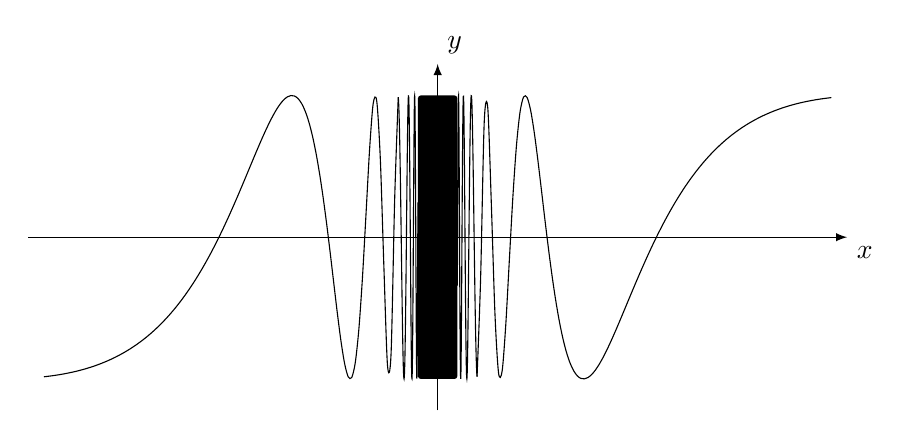
\begin{tikzpicture}[scale = 0.5]
\draw [-latex] (-10.4,0) -- (10.4,0) node [below right] {$x$};
\draw [-latex] (0,-4.4) -- (0,4.4) node [above right] {$y$};
\def \sc {1000};
\draw plot[domain=-10:-1, smooth, samples=100] (\x, {3.6*sin(\sc/\x)});
\draw plot[domain=-1:-0.5, smooth, samples=100] (\x, {3.6*sin(\sc/\x)});
\draw plot[domain=1:10, smooth, samples=100] (\x, {3.6*sin(\sc/\x)});
\draw plot[domain=0.5:1, smooth, samples=100] (\x, {3.6*sin(\sc/\x)});
\fill [rounded corners=1pt] (-0.5,-3.6) rectangle (0.5,3.6);
\end{tikzpicture}
\end{enumerate}
\paragraph{Def. 4:} Die Funktion $f: DB(f) \to \mathbb{R}, \; Db(f) \subseteq \mathbb{R}$ heißt
\begin{enumerate}[label=\alph*.)]
\item \emph{in einem Intervall $I \subset Db(f)$ stetig}, falls $f$ an jeder inneren Stelle $x_0 \in I$ stetig ist und in evtl. zu $I$ gehörenden Randpunkten einseitig stetig ist.
\item \emph{stetig}, falls $f$ in allen Punkten $x_0\in Db(f)$ stetig ist.
\end{enumerate}
\subparagraph{Bemerkung:} Jede der in 1.4.1 und 1.4.3 betrachteten Funktionen ist stetig.
\subparagraph{Bsp. 7:} $f: \mathbb{R}\setminus \{0\} \to \mathbb{R}, \; f(x)=\frac{1}{x}$ ist stetig.

\paragraph{Satz 3:} Sind $f$ und $g$ stetig in $x_0$, so sind auch $c_1 \cdot f + c_2 \cdot g, \; f\cdot g$ und $\frac{f}{g}$(falls $g(x_0)\not = 0$) stetig in $x_0$.

\paragraph{Satz 4:} (Stetigkeit und Verknüpfungen)\\
Seien $g: Db(g) \to \mathbb{R}$ und $f: Db(f) \to \mathbb{R}$ Funktionen mit $Wb(g)\subseteq Db(f)$, dann gilt:\\
Ist $g$ stetig in $x_0$ und $f$ stetig in $g(x_0)$, so ist $f\circ g:Db(g) \to \mathbb{R}, \; (f\circ g)(x) = f(g(x))$ stetig in $x_0$.

\paragraph{Satz 5:} (Zwischenwertsatz)\\
Sei $f: Db(f) \to \mathbb{R}, \; Db(f)\subseteq \mathbb{R}$ stetig auf $[a,b]  Db(f)$. Falls $f(a) \cdot f(b) < 0$ (also haben unterschiedliche Vorzeichen), so gilt $\exists x^*\in [a,b]$ mit $f(x^*)=0$\\
\begin{tikzpicture}[scale = 0.5]
\draw [-latex] (-6.4,0) -- (6.4,0) node [below right] {$x$};
\draw [-latex] (0,-4.4) -- (0,4.4) node [above right] {$y$};

\fill  (0.5,-2.5) circle (0.1);
\fill  (5.5,3.5) circle (0.1);
\draw  plot[smooth, tension=.7] coordinates {(0.5,-2.5) (1.5,-1.5) (2,-0.5) (3,0) (3.5,2) (4.5,3) (5.5,3.5)};

\draw (0.75,-0.5) -- (0.5,-0.5) -- (0.5,0.5) -- (0.75,0.5) node[above]{$a$};
\draw (5.5,0.5) node[above]{$b$} -- (5.75,0.5) -- (5.75,-0.5) -- (5.5,-0.5);
\draw (3,0.25) -- (3,-0.25) node[below]{$x^*$};
\draw (0.25,-2.5) -- (-0.25,-2.5) node[left]{$f(a)$};
\draw (0.25,3.5) -- (-0.25,3.5) node[left]{$f(b)$};
\end{tikzpicture}
\paragraph{Satz 6:} Sei $f: Db(f) \to \mathbb{R}, \; Db(f) \subseteq \mathbb{R}$ stetig auf $[a,b]$. Dann nimmt $f$ auf $[a,b]$ Minimum und Maximum an.

\subparagraph{Diskussion:}
\begin{enumerate}[label=\alph*.)]
\item $f(x) = \tan x$ nimmt auf $\left( - \frac{\pi}{2}, \frac{\pi}{2}\right)$ kein Maximum an.\\
\begin{tikzpicture}[scale = 0.5]
\draw plot [domain=(-1.3):(1.3)] (\x, {tan(\x r)} );
\draw (1.56, 0.2) -- (1.56, -0.2) node [below]{$\frac{\pi}{2}$};
\draw (-1.56, 0.2) -- (-1.56, -0.2) node [below]{$-\frac{\pi}{2}$};

\draw [-latex] (-3.2*2,0) -- (3.2*2,0) node [below right] {$x$};
\draw [-latex] (0,-2.2*2) -- (0,2.2*2) node [above right] {$y$};
\end{tikzpicture}
\item $f(x) = \begin{cases}
\arctan \frac{1}{x} & x \in [-1,1]\setminus \{0\}\\
0 & x = 0
\end{cases}$ nicht stetig und nimmt kein Maximum auf $[-1,1]$ an.\\
\begin{tikzpicture}[scale = 0.5]
\draw [-latex] (-6.4,0) -- (6.4,0) node [below right] {$x$};
\draw [-latex] (0,-4.4) -- (0,4.4) node [above right] {$y$};
\draw plot[domain=-5:-0.01, smooth] (\x, {-2.7^(\x)-1});
\draw plot[domain=0.01:5, smooth] (\x, {2.7^(-\x)+1});
\draw  (0,2) circle (0.2);
\draw  (0,-2) circle (0.2);
\fill  (0,0) circle (0.2);
\end{tikzpicture}
\end{enumerate}

\section{Potenzreihen}
\paragraph{Def.:} Sei $(a_n)$ eine Zahlenfolge und $x_0 \in \mathbb{R}$ heißt $\boxed{\sum_{n=0}^\infty a_n (x-x_0)^n}$ Potenzreihe mit dem Mittelpunkt $x_0$.
\subparagraph{Diskussion:} 
\begin{itemize}
\item Für jedes feste $x \in \mathbb{R}$ ist die Potenzreihe eine feste Reihe.
\item Konvergenzbereich $K:=\{x\in \mathbb{R} | \text{Potenzreihe ist konvergent}\}$
\item Für jedes $x\in K$ existiert der Summenwert der Potenzreihe. Die Funktion $f: K \to \mathbb{R}$ mit $f(x) = \sum_{n=0}^\infty a_n (x-x_0)^n$ heißt Grenzfunktion der Potenzreihe.
\end{itemize}
Zur Bestimmung des Konvergenzbereichs nutz man Satz 10 und 11 aus \ref{2.1.3} und erhält absolute Konvergenz in einem um $x_0$ liegendem Konvergenzintervall $I:=(x_0-r, x_0+r)$.\\
Wie $r$ bestimmt wird liefert:

\paragraph{Satz 1:} Sei $(a_n)$ Zahlenfolge mit $r:=\lim_{n\to \infty} \left| \frac{a_n}{a_{n+1}}\right|=\lim_{n\to \infty} \frac{1}{\sqrt[n]{|a_n|}}$ existiert.\\
Dann ist $\sum_{n=0}^\infty a_n (x-x_0)^n\begin{cases}
\text{absolut konvergent} & \text{für }x\in \mathbb{R} \text{ mit }|x-x_0|<r\\
\text{divergent} & \text{für }x\in \mathbb{R} \text{ mit }|x-x_0|>r
\end{cases}$.\\
\begin{tikzpicture}[scale = 0.7]
\draw (0,0.25) -- (0,-0.25) node[below]{$x_0$};
\draw (3,0.25) -- (3,-0.25) node[below]{$x_0+r$};
\draw (-3,0.25) -- (-3,-0.25) node[below]{$x_0-r$};
\draw [(-), green, thick](-3,0.1) -- (3,0.1) node [above, pos=0.5]{absolut konvergent};
\draw [-), orange, thick](-6,0.1) -- (-3,0.1) node [above, pos=0.5]{divergent};
\draw [(-, orange, thick](3,0.1) -- (6,0.1) node [above, pos=0.5]{divergent};
\draw [-latex] (-6.4,0) -- (6.4,0) node [below right] {$x$};
\end{tikzpicture}

\subparagraph{Diskussion:} 
\begin{itemize}
\item Verwechslungsgefahr:
\begin{itemize}
\item Satz 10 und 11 betrachten (Zahlen-)Reihen $\sum_{n=0}^\infty a_n$
\item Satz 1 betrachtet Potenzreihen $\sum_{n=0}^\infty a_n (x-x_0)^n$, wobei $a_n$ ein Faktor vor $(x-x_0)^n$ ist.
\end{itemize}
\item Falls der Grenzwert $r$ aus Satz 1 nicht existiert, so gibt es trotzdem einen Konvergenzradius.\\
Den gilt es auf andere Weise zu betrachten/ermitteln.
\item Satz 1 sagt nichts über das Verhalten an den Randpunkten aus $\rightarrow$ gesonderte Untersuchung nötig.
\end{itemize}
\subparagraph{Bsp. 1:} 
\begin{enumerate}[label=\alph*.)]
\item $\sum_{n=1}^\infty \frac{x^n}{n}$, d.h. $x_0=0$, $a_n=\frac{1}{n}$, $n=1,2,...$\\
$r= \lim_{n\to\infty} \frac{1}{\sqrt[n]{\left|\frac{1}{n}\right|}}=\lim_{n\to \infty}=\frac{1}{\frac{1}{\sqrt[n]{n}}}=\lim_{n\to\infty}\sqrt[n]{n}=1$\\
$\Rightarrow$ Konvergenzintervall $I=(-1,1)$\\
Randpunkte:\\
$x=-1: \sum_{n=1}^\infty \frac{(-1)^n}{n}$ bedingt konvergent (alternierenden harmonische Reihe)\\
$x=1: \sum_{n=1}^\infty \frac{1}{n}$ divergent\\
$\Rightarrow$ Konvergenzbereich: $K=[-1,1)$
\item $\sum_{n=0}^\infty \frac{x^n}{n!}$, d.h. $x_0=0$, $a_n=\frac{1}{n!}$\\
$\left| \frac{a_n}{a_{n+1}}\right| = \frac{\frac{1}{n!}}{\frac{1}{(n+1)!}}=\frac{(n+1)!}{n!}=n+1\overset{n\to \infty}{\longrightarrow} \infty$\\
$\Rightarrow r = \infty$\\
d.h. die Reihe ist absolut konvergent für alle $x \in \mathbb{R}$.\\
Bezeichnung: \emph{beständige Konvergenz}
\item $\sum_{n=0}^\infty \frac{x^{2n}}{(2n)!}=1+\frac{x^2}{2!}+\frac{x^2}{4!}+...\quad$ d.h. $x_0 = 0$, $a_n=\begin{cases}
\frac{1}{n} & n \text{ gerade}\\
0 & n \text{ungerade}
\end{cases}$\\
Satz 1 ist aber nicht unmittelbar anwendbar.\\
Substitution $u:=x^2$ liefert aber $\sum_{n=0}^\infty \frac{u^n}{(2n)!}$ mit $u_0=0$, $b_n=\frac{1}{(2n)!}$ ($\sum b_n (u-u_0)^n$)\\
$\left| \frac{b_n}{b_{n+1}}\right|=\frac{(2n+2)!}{(2n)!}=(2n+2)\cdot (2n+1) \overset{n\to \infty}{\longrightarrow} \infty$\\
$\Rightarrow r_u=\infty$ (Konvergenzradius für die Substituierte Reihe)\\
$\Rightarrow r_x=\mq{\sqrt{\infty}\,}= \infty$ (Konvergenzradius für die untersuchte Funktion)\\
Im Konvergenzbereich $K$ wird dadurch eine Potenzreihe eine Funktion dargestellt, die Grenzfunktion (siehe vorhergehende Diskussion).
\end{enumerate}
\subparagraph{Bsp. 2:}
\begin{enumerate}[label=\alph*.)]
\item $\sum_{n=0}^\infty x^n = \frac{1}{1-x}$ für $x\in (-1,1)$ (geometrische Reihe)
\item $\sum_{n=0}^\infty \frac{x^n}{n!}=e^x$ für $x\in \mathbb{R}$ (Beweis später)
\end{enumerate}
\paragraph{Satz 2:} Die \emph{Grenzfunktion} jeder Potenzreihe ist \emph{im Konvergenzbereich stetig}.